\documentclass[12pt, oneside]{article}
 
\usepackage{graphicx}
\usepackage{hyperref}
\graphicspath{ {Images/} }

\begin{document}
\thispagestyle{empty}
\begin{center}
\begin{minipage}{0.75\linewidth}
    \centering

    {\uppercase{\Large COS 301 Assignment\par}}
   	{\uppercase{\Large Group 5 B \par}}
    \vspace{1cm}
    
\includegraphics[scale=0.3]{example} %Example is the name of the image

    {\normalsize Firdous Tayob (13098472)\par}
    {\normalsize Sebastian Gerber (12213749)\par}
    {\normalsize Godfrey Mathe (13103394)\par}
    {\normalsize Shaun Meintjies (13310896)\par}
    {\normalsize Duran Cole (13329414)\par}
    {\normalsize Isabel Nel (1307030)\par}
    \vspace{1cm}
    
    {\Large February 2015}
\end{minipage}
\end{center}
\clearpage

\newpage

\section{Introduction}
	Fill in later...
	
\section{Vision}
	Fill in later...
	
\section{Background}
	\begin{enumerate}
		\item List example
		\item List example
		\item List example
		\item List example
		\item List example
	\end{enumerate}
	
\section{Architecture requirements}
	\subsection{Access channel requirements}
		Fill in later...
	\subsection{Quality requirements}
		Fill in later...
	\subsection{Integration requirements}
		Fill in later...
	\subsection{Architecture constraints}
		Fill in later...
	
\section{Functional requirements and application design}
	\subsection{Use case prioritization}
		\subsubsection{Critical}
			\begin{itemize}
				\item Login
				\item Logout
				\item Post
				\item Thread
				\item Buzz Space
			 \end{itemize}
		\subsubsection{Important}
			\begin{itemize}
				\item Search
				\item Voting
			 \end{itemize}
		\subsubsection{Nice to Have}
			\begin{itemize}
				\item Request
				\item Voting
			 \end{itemize}
	\subsection{Use case/Services contracts}
			\subsubsection{Login}
				Pre-Conditions : \begin{itemize}
							\item Must not be logged in.
						     \end{itemize}
				Post-Conditions : \begin{itemize}
							\item If login succesful, user will be logged in.
							\item If login failed. user will be asked to resubmit
						     \end{itemize}
			\subsubsection{Logout}
				Pre-Conditions : \begin{itemize}
							\item Must be logged in.
						     \end{itemize}
				Post-Conditions : \begin{itemize}
							\item User is logged out.
						     \end{itemize}
			\subsubsection{CreatePost}
				Pre-Conditions : \begin{itemize}
							\item Must be logged in.
							\item A thread should exist.
						     \end{itemize}
				Post-Conditions : \begin{itemize}
							\item Post is created.
						     \end{itemize}
   				 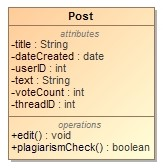
\includegraphics[scale=1]{CreatePost}
			\subsubsection{Request}
				Pre-Conditions : \begin{itemize}
							\item Must be logged in.
						     \end{itemize}
				Post-Conditions : \begin{itemize}
							\item Request is sent.
						     \end{itemize}
   				 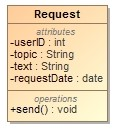
\includegraphics[scale=1]{Request}
			\subsubsection{Thread}
				Pre-Conditions : \begin{itemize}
							\item Only Authorised persons may use this functionality
							\item Buzz Space needs to exist 
							\ No such thread sould already exist
						     \end{itemize}
				Post-Conditions : \begin{itemize}
							\item A new Thread now exists under which people can create posts
						     \end{itemize}
			\subsubsection{Voting}
				Pre-Conditions : \begin{itemize}
							\item Must not be logged in.
							\item User has not yet voted
						     \end{itemize}
				Post-Conditions : \begin{itemize}
							\item User voted
						     \end{itemize}	

	\subsection{Required functionality}
		Use case diagram for a thread
		
			 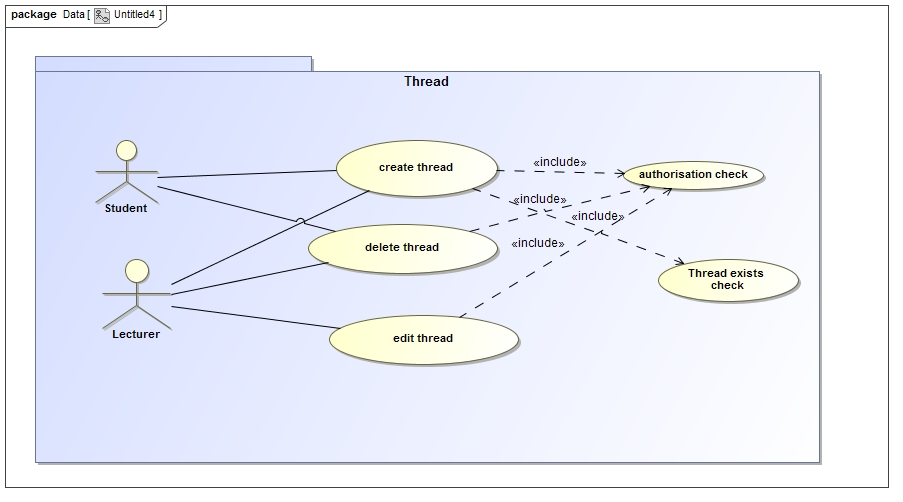
\includegraphics[scale=1]{thread}
			 
		Use case diagram for a post
		
			 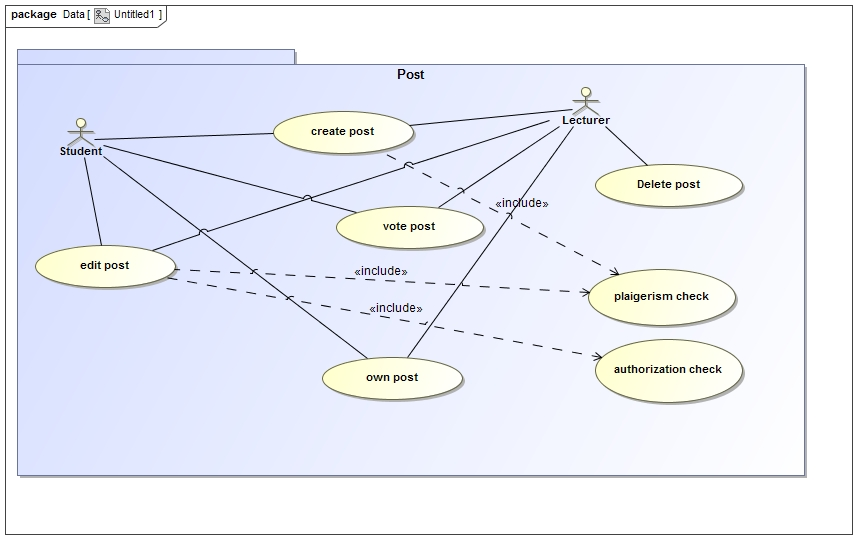
\includegraphics[scale=1]{post}
			 
		Use case diagram for a request
		
			 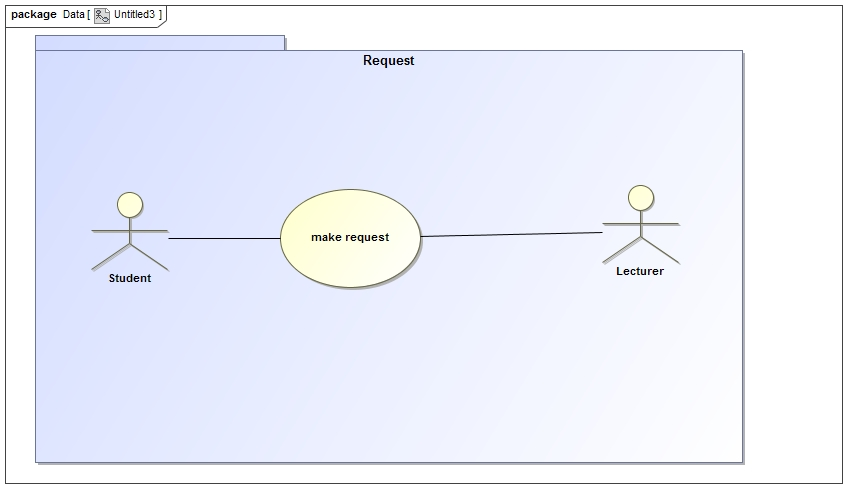
\includegraphics[scale=1]{request1}
			 
	\subsection{Process specifications}
		Put words here...
	\subsection{ Domain Model}
		Put words here...




\end{document}